\begin{surferPage}[منحنى بارت المسدس]{منحنى بارت المسدس}
    تم بناء هذا المنحنى من الدرجة $ 6 $ (مسدس) من قبل وولف بارت 
    \textenglish{(Wolf Barth)} في 1996. 
    
  يملك منحنى بارت المسدس $ 65 $ نقطة متفردة.
    بعد وقت كثير من بناء بارت، أثبت كل من جاف 
    \textenglish{(Jaffe)}
     وروبرمان
    \textenglish{(Ruberman)}
     أن هذا هو أكبر عدد نقاط متفردة محتمل في منحنى مسدس. أي أنه لا يمكن تحطيم رقم بارت القياسي!


    أتى بناء بارت كمفاجئة كبيرة لأنه لوقت طويل ساد الإعتقاد أن المنحنيات من الدرجة $ 6 $ تملك $ 64 $ نقطة متفردة فقط.

    
 ميزة لافتة للنظر في بناء بارت وهي أنه يملك تناظر متعدد أسطح ذي 20 وجهاً:
 تظهر الصورة متعدد أسطح ذا 20 وجهاَ ومستوياته التناظرية:
   
  \begin{center}
      \vspace*{-0.1cm}
      \begin{tabular}{@{}c@{\ \ }c@{\,}c@{}}
        \begin{tabular}{@{}c}
          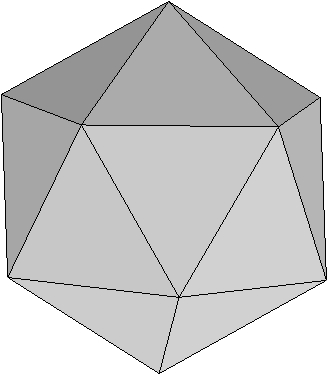
\includegraphics[width=1.4cm]{./../../common/images/icosah}
        \end{tabular}
        &
        \begin{tabular}{@{}c}
          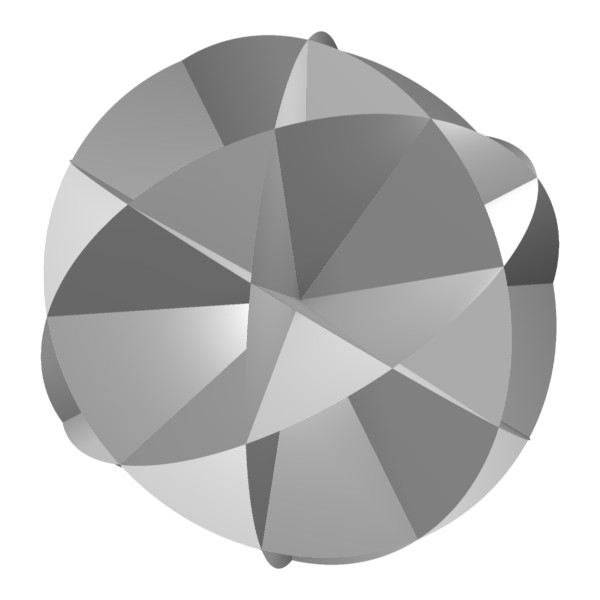
\includegraphics[width=1.4cm]{./../../common/images/barth_sextic_planes}
        \end{tabular}
        &
        \begin{tabular}{c@{}}
          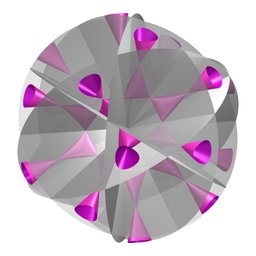
\includegraphics[width=1.4cm]{./../../common/images/barth_sextic_and_planes}
        \end{tabular}
      \end{tabular}
    \end{center}
    \vspace*{-0.1cm}

    يحقق منحنى بارت المسدس المعادلة
    $P_6 - \alpha K^2=0,$
     حيث $P_6$
    تشير إلى مستويات التناظر الستة
    وحيث 
     $K=x^2+y^2+z^2-1$ 
     هي كرة الوحدة وحيث 
    $\alpha=\frac{1}{4}(2+\sqrt{5})$.
\end{surferPage}